\chapter[Introdução]{Introdução}

\section{Contexto}

\section{Objetivos}

\chapter{Referencial teórico}

\section{Diagrama entidade-relacionamento}
Segundo \citeonline{projetobancodedados} , a abordagem mais utilizada e conhecida é a 
entidade-relacionamento (ER) onde o modelo de dados é geralmente representado graficamente através
de um diagrama entidade-relacionamento (DER). Esta abordagem foi criada em 1976 por Peter Chen e
é considerada como um padrão para a modelagem conceitual.

A abordagem entidade-relacionamento é baseada em dois principais pilares que são apresentados em seguida.

\subsection{Entidade}
De acordo com \citeonline{projetobancodedados}, uma entidade, no modelo conceitual, representa um conjunto
de objetos da realidade modelada. Seu principal objetivo é modelar de forma abstrata um banco de dados, onde
se te interesse somente nos objetos sobre os quais deseja-se manter informações. No DER, uma entidade é representada
por meio de um retângulo contendo o nome da entidade.
 
\subsection{Relacionamento}
Como apresentado por \citeonline{projetobancodedados}, o DER permite a especificar as propriedades dos objetos
que serão armazenados no banco de dados, como por exemplo o relacionamento/associação entre os objetos. No DER,
um relacionamento é representado por meio de um losango que são ligados por linhas aos retângulos que representam
as entidades que participam de um determinado relacionamento.

Na figura \ref{figura1} é apresentado um exemplo simples de um diagrama entidade-relacionamento (DER). É possível notar 
no diagrama a existência de atributos e cardinalidade, estes dois são apresentados logo em seguida.

\begin{figure}[h]
	\centering
	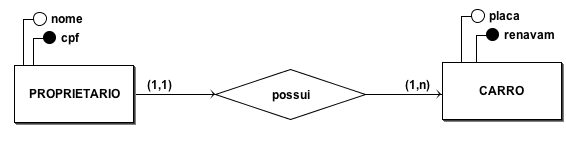
\includegraphics[keepaspectratio=true,scale=0.5]{figuras/figura1.png}
	\caption{Exemplo de DER}
	Fonte: Autor
	\label{figura1}
\end{figure}

Os atributos correspondem às características/qualidades que descrevem uma entidade, são representados por
elipses ou círculos acompanhados por seus respectivos nomes \cite{sistemadebancos}.

As cardinalidades representam a restrição do número de objetos que podem participar do relacionamento. Na notação
de Peter Chen, as cardinalidade são apresentadas próximas às ligações de relacionamento e são compostas da quantidade
mínima e máxima de objetos que podem participar do relacionamento. Tais características podem ser vistas 
na figura \ref{figura1} \cite{sistemadebancos}.



\chapter{Ferramenta gamificada de apoio ao ensino e aprendizagem de programação}

\chapter{Implementação da solução}

\section{Modelagem de dados}

\begin{figure}[h]
	\centering
	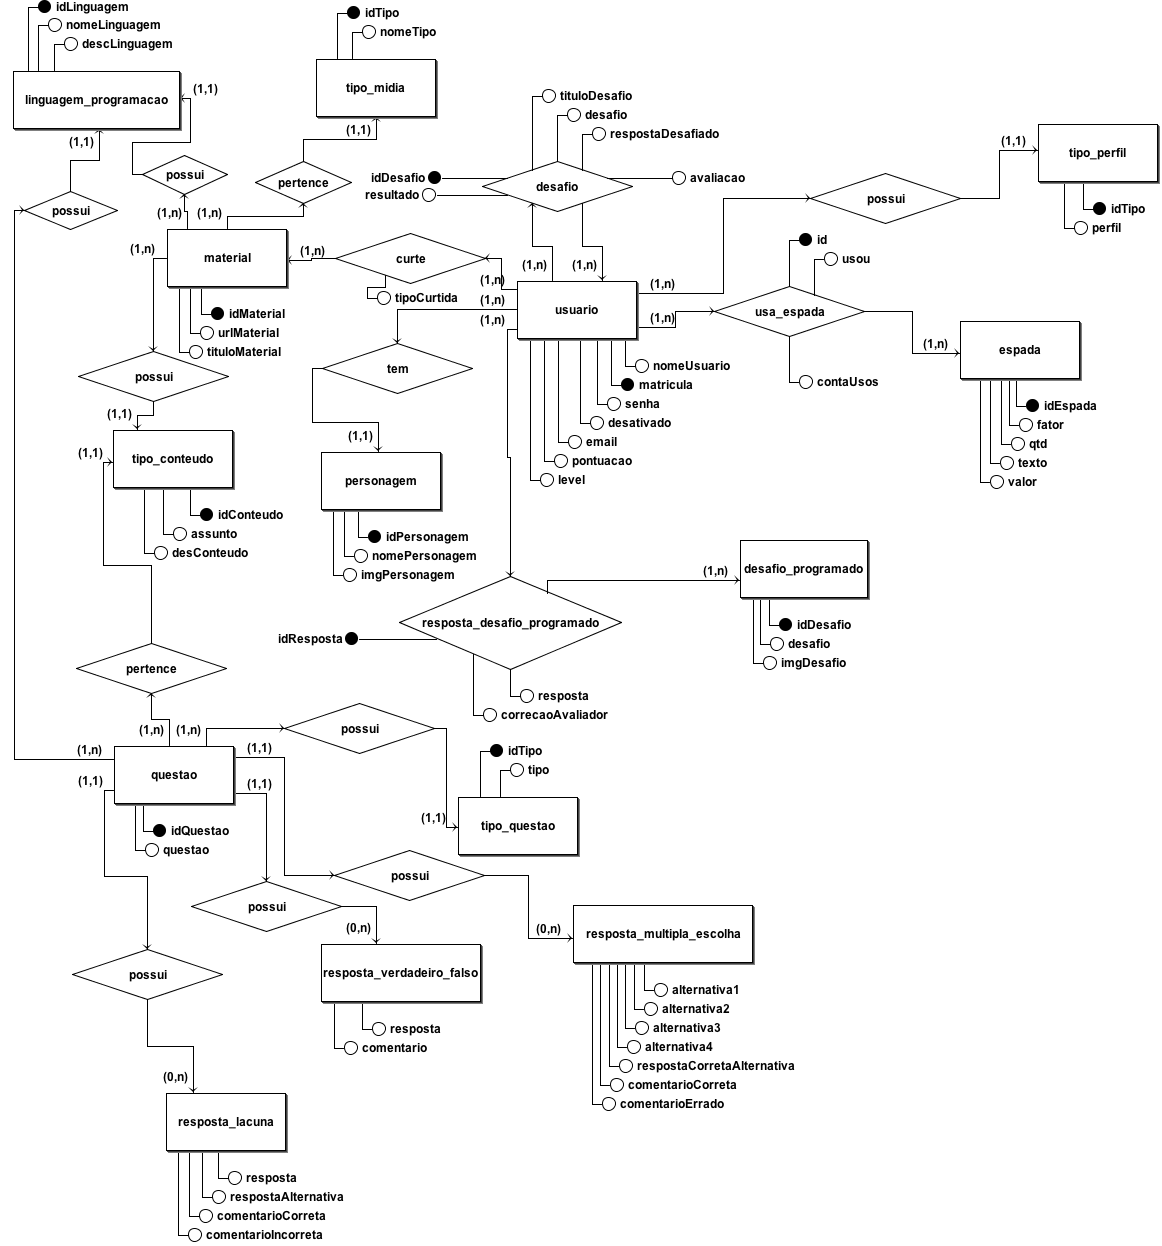
\includegraphics[keepaspectratio=true,scale=0.4]{figuras/der.png}
	\caption{DER da ferramenta}
	Fonte: Autor
	\label{figura2}
\end{figure}


\begin{figure}[h]
	\centering
	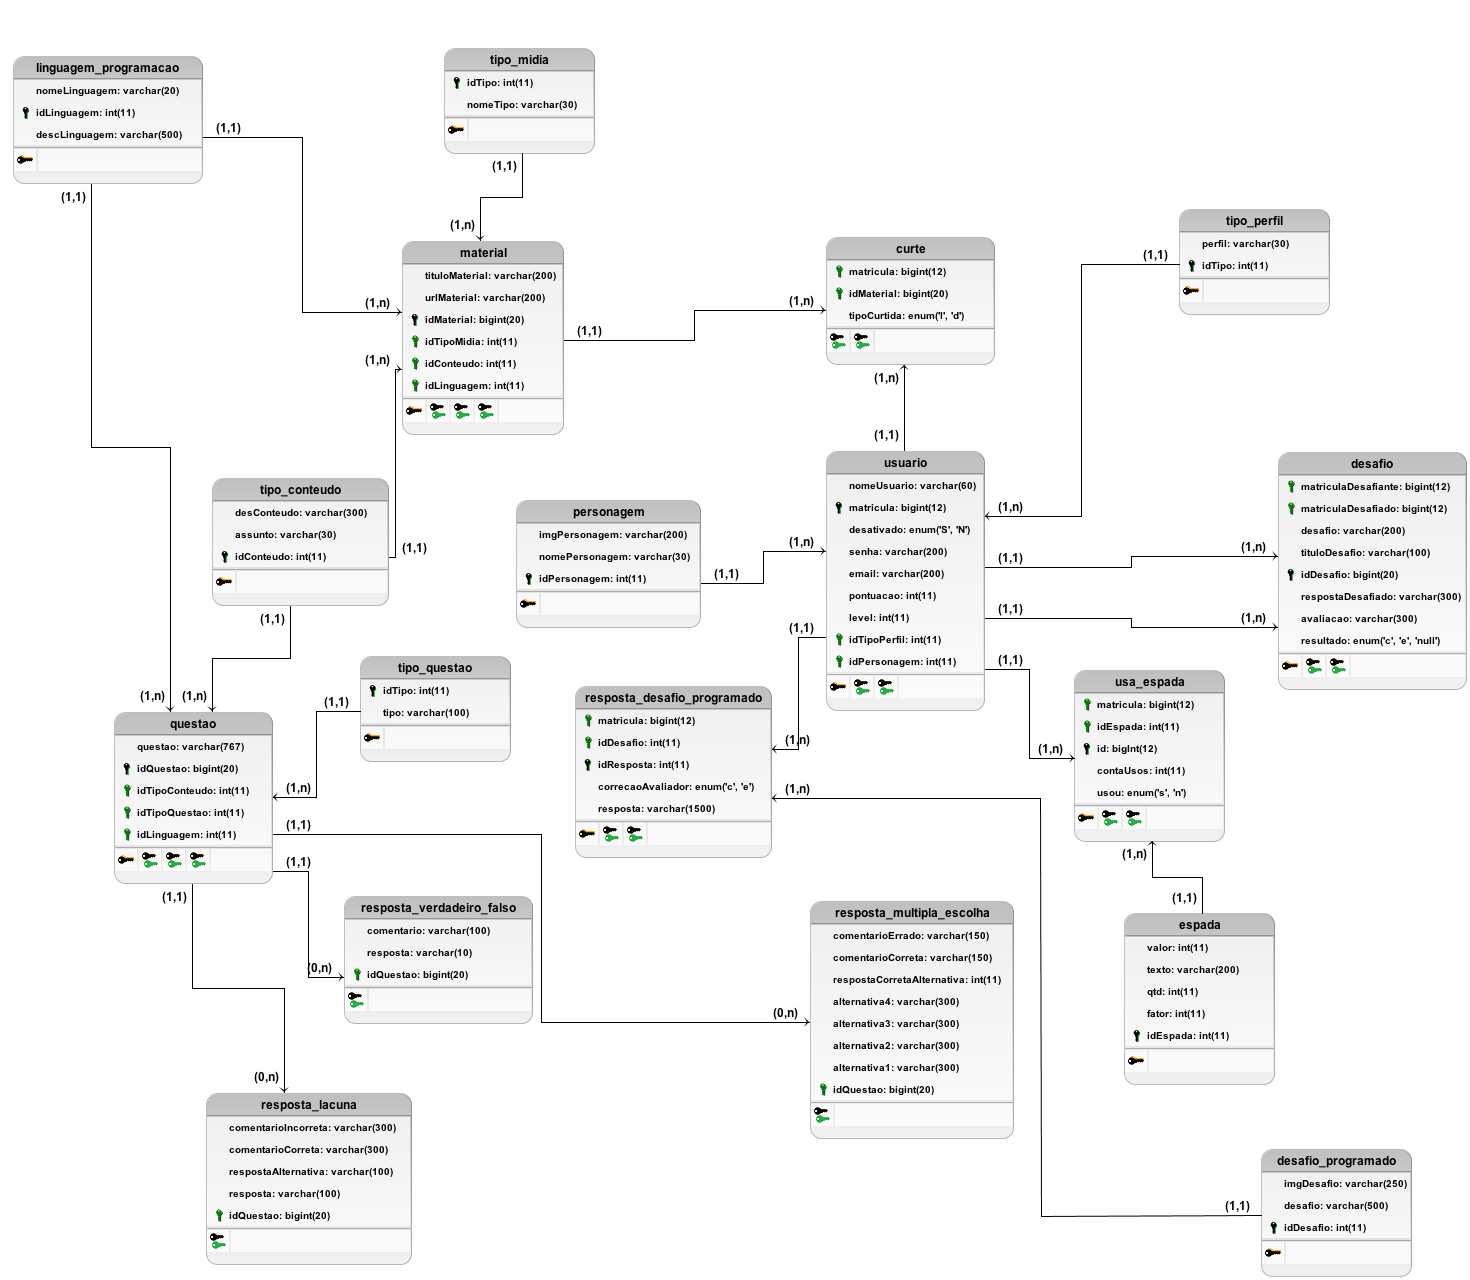
\includegraphics[keepaspectratio=true,scale=0.32]{figuras/dl.png}
	\caption{DL da ferramenta}
	Fonte: Autor
	\label{figura3}
\end{figure}


\chapter{Narrativa}

\section{Contexto}

Com o objetivo de aumentar o engajamento dos estudantes/jogadores, fora desenvolvida uma história que se passa em um mundo 
onde criaturas (Orcs) invadem o vilarejo do jogador que, motivado pelo desejo de vingança e tendo sido escolhido entre uma legião 
de outros guerreiro, dá início à jornada onde o mesmo deve cumprir com desafios como: quiz, desafiar outros jogadores entre outras
atividades que dão ao jogador pontos que podem ser trocados por itens ou serem acumulados afim de obter boas posições nos \textit{rankings}.

\section{Personagens}